% --- To be compiled with XeLaTeX ---
% ---      Encoding: UTF-8        ---

\documentclass[a4paper, oneside, 11pt]{article}

%fontspec package provides a configurable interface for font selection, and allows complex font choices to be named and later reused. It's needed for XeLaTeX
\usepackage[cm-default]{fontspec}

% Unicode support
\usepackage{xunicode}
\usepackage{xltxtra}

% Default words and phrases in Greek (e.g. 'Περίληψη' instead of 'Abstract'). Also contains hyphenation rules for Greek Language
\usepackage{xgreek}

% Mathematical fonts, theorems etc.
\usepackage{amsfonts}
\usepackage{amsmath}
\usepackage{amsthm}

% Default page layout for consuming a larger portion of the page.
\usepackage{fullpage}

% Greek fonts (Computer Modern)
\setmainfont[Mapping=tex-text]{CMU Serif}

% Auxiliary commands
\newcommand{\HRule}{\rule{\linewidth}{0.5mm}}

\newtheorem{thm}{Θεώρημα}
\newtheorem{lm}[thm]{Λήμμα}
\newtheorem{obsrv}[thm]{Παρατήρηση}

\theoremstyle{definition}
\newtheorem{defn}[thm]{Ορισμός}

%\usepackage{subfigure}
\usepackage{graphicx}
\usepackage{caption}
\usepackage{subcaption}

\newcommand{\vc}{\text{vc}}

\begin{document}

\begin{titlepage}
\begin{center}


\includegraphics[width=0.3\textwidth]{/home/makis/.vim/skel/pyrforos.png}\\[1cm]

\textsc{\LARGE Σχολή Ηλεκτρολόγων Μηχανικών και Μηχανικών Υπολογιστών}\\[1.5cm]

\HRule \\[0.4cm]
{\huge \bfseries Γραφοθεωρία\\
\LARGE Ομάδα Ασκήσεων No. 1}\\[0.4cm]

\HRule \\[1.5cm]

\begin{center}
\textbf{Ομάδα 7}\\
Αξιώτης Κυριάκος\\
Αρσένης Γεράσιμος
\end{center}

\vfill

{\large \today}
\end{center}

\end{titlepage}


\section{Χρωματισμοί κορυφών και ακμών}
\begin{enumerate}
   \item[1.6] \emph{Έστω $G$ γράφημα όπου $\Delta(G) \leq 3$. Δείξτε ότι το
              $G$ είναι 4-ακμοχρωματίσιμο.}

   Θα δείξουμε ότι γραμμικό γράφημα $L(G)$ του $G$ είναι 4 χρωματίσιμο.

   Από το Θεώρημα Brooks έχουμε ότι το $L(G)$ θα είναι
   $\Delta(L(G))$-χρωματίσιμο εκτός αν είναι περιττός κύκλος
   ή κλίκα όπου σε αυτή την περίπτωση θα είναι $(\Delta(L(G)) + 1)$-χρωματίσιμο.

   Αν το $L(G)$ είναι περιττός κύκλος τότε θα είναι 3-χρωματίσιμο.

   Αν είναι κλίκα με 3 ή λιγότερες κορυφές τότε προφανώς είναι
   3-χρωματίσιμο ενώ αν είναι κλίκα με τουλάχιστον 4 κορυφές τότε
   περιέχει το $K_4$ ως υπογράφημα όμως αυτό δεν γίνεται
   σύμφωνα με το Λήμμα \ref{lm1.6.1}.

   Επομένως το $L(G)$ θα είναι $\Delta(L(G))$-χρωματίσιμο και από
   την Παρατήρηση \ref{lm1.6.2} συμπεραίνουμε ότι θα είναι
   4-χρωματίσιμο.
   
   \begin{lm}
      \label{lm1.6.1}
      Αν $K_4 \subseteq L(G)$ τότε $\Delta(G) \geq 4$.
   \end{lm}
   \begin{proof}
      Έστω $e_1, e_2, e_3, e_4$ οι ακμές του $G$ που στο $L(G)$ είναι
      κορυφές 4-κλίκας. Αυτό σημαίνει ότι κάθε ζεύγος $e_i, e_j$ θα πρέπει
      να έχει κοινό άκρο.

      Έστω $e_1 = \{u, v\}$ και χωρίς βλάβη της γενικότητας έστω
      $e_2 = \{u, w\}$. Αν η $e_3$ έχει κοινό άκρο με την $e_1$
      την κορυφή $v$, τότε αναγκαστικά $e_3 = \{v, w\}$ ώστε να έχει
      κοινό άκρο και με την $e_3$. Σε αυτή την περίπτωση όμως η $e_4$
      δεν μπορεί να έχει κοινό άκρο και με τις 3 προηγούμενες ακμές.

      Άρα η $e_3$ έχει κοινό άκρο με την $e_1$ το $u$, δηλαδή
      $e_3 = \{ u, x \}$ για κάποια κορυφή $x$ (διαφορετική από
      τις $\{u, v, w\}$).

      Τέλος, η $e_4$ θα πρέπει να έχει κοινό άκρο με όλες τις υπόλοιπες
      και αυτό μπορεί να συμβεί μόνο αν $e_4 = \{u, y\}$ για κάποια
      νέα κορυφή $y$.

      Συνεπώς $\Delta(G) \geq d(u) = 4$.
   \end{proof}

   \begin{obsrv}
      \label{lm1.6.2}
      Αν $\Delta(G) \leq 3$ τότε $\Delta(L(G)) \leq 4$.
   \end{obsrv}
   \begin{proof}
      Έστω ότι υπήρχε ακμή $e = \{u, v\} \in E(G)$ η οποία να έχει κοινό
      άκρο με τουλάχιστον 5 άλλες ακμές στο $G$. Αυτό σημαίνει ότι
      σε ένα από τα άκρα της $e$, έστω στο $u$, θα προσπίπτουν τουλάχιστον
      3 από αυτές τις 5 ακμες και έτσι η $u$ θα έχει βαθμό τουλάχιστον
      4 το οποίο είναι άτοπο.
   \end{proof}

   \item[1.7] \emph{Δείξτε ότι υπάρχει $c$ τέτοιο ώστε κάθε ένωση δύο επίπεδων
              γραφημάτων να έχει χρωματικό αριθμό το πολύ $c$.}
   
   \begin{lm}
      \label{lm1.7.1}
      Αν $G = G_1 \cup G_2$ τότε $\chi(G) \leq \chi(G_1) \cdot \chi(G_2)$.
   \end{lm}
   \begin{proof}
      Έστω $\chi(G_1) = k, \chi(G_2) = l$
      και $\chi_{G_1} : V(G_1) \rightarrow [k],
      \chi_{G_2} : V(G_2) \rightarrow [l]$ οι συναρτήσεις
      χρωματισμού του καθενός.
      
      Επεκτείνουμε τις παραπάνω συναρτήσεις ως εξής:
      \[ \overline{\chi_{G_i}}(u) = \left\{
         \begin{array}{cc}
            \chi_{G_i}(u) & ,\ u \in V(G_i)\\
            1 & , \text{ διαφορετικά}
         \end{array}
         \right.
      \]

      Ορίζουμε το σύνολο $S = \{ (x, y)\ |\ x \in A, y \in B \}$ και
      χρωματίζουμε το $G$ με χρώματα από το $S$ ως εξής:

      \[ \chi_G(u) = \left( \overline{\chi_{G_1}}(u),
                     \overline{\chi_{G_2}}(u) \right) \]

      Ο παραπάνω είναι έγκυρος χρωματισμός αφού αν $\chi_G(u) = \chi_G(v)$
      τότε $\overline{\chi_{G_i}}(u) = \overline{\chi_{G_i}}(v)$
      για $i = 1, 2$ επομένως $\{ u, v \} \notin E(G_i)$ και έτσι
      $\{u, v\} \notin E(G)$.

      Άρα $\chi(G) \leq |S| = \chi(G_1) \cdot \chi(G_2)$.
   \end{proof}

   Από το θεώρημα των 4 χρωμάτων έχουμε ότι αν $G_1, G_2$ επίπεδα γραφήματα
   τότε $\chi(G_1), \chi(G_2) \leq 4$ επομένως από το Λήμμα \ref{lm1.7.1}:
   $\chi(G_1 \cup G_2) \leq 16$.
\end{enumerate}

\section{Διαπεράσεις}
\begin{enumerate}
   \item[2.1] \emph{$(\star)$ Για ποιά $k$ και $l$ το γράφημα
              $G_{k, l} = P_l^{[k]}$ είναι Χαμιλτονιανό;}

   Για $k = 1$, κανένα από τα $P_l$ με $l \geq 1$ δεν είναι Χαμιλτονιανό.

   Για $k \geq 2$, θα δείξουμε ότι το $P_l^{[k]}$ είναι Χαμιλτονιανό
   αν και μόνο αν το $l$ είναι άρτιος.

   \begin{obsrv}
      Το $P_l^{[k]}$ είναι ένα $k$-διάστατο πλέγμα (grid). Στο εξής
      θα αριθμούμε τις κορυφές του με βάση τις συντεταγμένες
      στις οποίες βρίσκονται, δηλαδή:

      \[ V(P_l^{[k]}) = \{ (x_1, \ldots, x_k)\ |\  1 \leq x_i \leq l \text{ για }
      1 \leq i \leq k \} \]

      Για τις ακμές έχουμε:

      \[ E(P_l^{[k]}) = \{ \{ (x_1, \ldots, x_k), (y_1, \ldots, y_k) \}
         \ |\ \exists i:\ (|x_i - y_i| = 1
         \land \forall j \neq i:\ x_j = y_j) \} \]
   \end{obsrv}

   \begin{obsrv}
      \label{lm2.1.1}
      Το $P_l^{[2]}$ για $l$ άρτιο είναι Χαμιλτονιανό.
   \end{obsrv}
   \begin{proof}
      Ξεκινάμε από την πάνω αριστερά κορυφή και διατρέχουμε τις
      κορυφές της πρώτης στήλης προς τα κάτω. Έπειτα διατρέχουμε
      από κάτω προς τα πάνω τις κορυφές της δεύτερης στήλης
      μέχρι τη γραμμή 2 και συνεχίζουμε έτσι μέχρι να διατρέξουμε
      από κάτω προς τα πάνω (επειδή το $l$ είναι άρτιο) τις κορυφές
      τις τελευταίας στήλης όπου και κλείνουμε τον κύκλο διατρέχοντας
      στο τέλος τις κορυφές της πρώτης γραμμής.
   \end{proof}

   \begin{lm}
      \label{lm2.1.2}
      Αν $G$ είναι Χαμιλτονιανό τότε το $G \times P_k$ είναι επίσης
      Χαμιλτονιανό.
   \end{lm}
   \begin{proof}
      Το γράφημα $G \times P_k$ είναι ουσιαστικά το $G$ όπου κάθε κορυφή του
      έχει αντικατασταθεί από ένα μονοπάτι $P_k$ (και έχουν προστεθεί οι
      κατάλληλες ακμές μεταξύ κορυφών των μονοπατιών).

      Ας πάρουμε ένα κύκλο Hamilton του $G$:
      
      \[ u_1 \rightarrow \ldots \rightarrow u_n \rightarrow u_1 \]

      Αυτός μπορεί να μετασχηματιστεί απευθείας
      σε κύκλο Hamilton του $G \times P_k$ ως εξής:
      
      \[ (u_1^1 \rightarrow \ldots \rightarrow u_1^k) \rightarrow
         \ldots \rightarrow (u_n^1 \rightarrow \ldots
         \rightarrow u_n^k) \rightarrow u_1^1 \]

      όπου στο παραπάνω $u_i^j$ είναι η $j$-οστή κορυφή του μονοπατιού
      το οποίο έχει αντικαταστήσει την κορυφή $u_i$ του $G$ στον
      $G \times P_k$.
   \end{proof}

   Από το Λήμμα \ref{lm2.1.2} και την Παρατήρηση \ref{lm2.1.1} έχουμε
   επαγωγικά ότι για κάθε $k \geq 2$ και για $l$ άρτιο το $P_l^{[k]}$
   είναι Χαμιλτονιανό.

   \begin{lm}
      \label{lm2.1.3}
      Αν $l$ περιττός τότε το $G = P_l^{[k]}$ \emph{δεν} είναι Χαμιλτονιανό.
   \end{lm}
   \begin{proof}
      Ορίζουμε την εξής διαμέριση των κορυφών του $G$
      σε δύο σύνολα $A_1, A_2$:

      \[ A_i = \left\{ (x_1, \ldots, x_k) \in V(G)\ |\
               \sum_{i=j}^{k} x_j \equiv i \pmod{2} \right\}
               \text{ για } i = 1, 2\]

      Είναι φανερό ότι δεν υπάρχει ακμή μεταξύ κορυφών που βρίσκονται
      στο ίδιο σύνολο γιατί τα αθροίσματα των συντεταγμένων γειτονικών κορυφών
      διαφέρουν ακριβώς κατά ένα.

      Παρατηρούμε επίσης ότι το $G$ έχει $l^k$ κορυφές το οποίο είναι
      περιττός αριθμος για $l$ περιττό επομένως ένα από τα δύο
      σύνολα $A_1, A_2$ θα είναι μεγαλύτερο από το άλλο. Χωρίς βλάβη
      της γενικότητας υποθέτουμε $|A_1| > |A_2|$.

      Θεωρούμε λοιπόν το γράφημα $G \backslash A_2$ το οποίο
      θα πρέπει να έχει $|A_1| > |A_2|$ συνεκτικές συνιστώσες αποτελούμενες
      από μία κορυφή η κάθε μία. Όπως δείχνουμε όμως στην άσκηση
      2.10, ένα τέτοιο γράφημα δεν μπορεί να είναι Χαμιλτονιανό.
   \end{proof}


   \item[2.7] \emph{$(\star)$ Έστω $G$ συνεκτικό γράφημα τέτοιο ώστε το συμπλήρωμά του να είναι ατρίγωνο. Δείξτε ότι το $G$ έχει Χαμιλτονιανό μονοπάτι}

Έστω το μέγιστο μονοπάτι στο γράφημα. Αν όλες οι κορυφές είναι πάνω σε αυτό το μονοπάτι, έχουμε τελειώσει. Διαφορετικά, υπάρχει μια κορυφή $u$ που είναι έξω από το μονοπάτι. Η $u$ δεν μπορεί να έχει
ακμή προς κάποιο από τα δύο άκρα του μονοπατιού, αφού τότε θα είχαμε άτοπο στη μεγιστότητα του μονοπατιού. Επειδή όμως το συμπλήρωμα είναι ατρίγωνο, θα πρέπει να υπάρχει ακμή μεταξύ των δύο ακρών
του μονοπατιού, έχουμε δηλαδή έναν κύκλο $C$. Τώρα, επειδή το γράφημα είναι συνεκτικό, θα υπάρχει ακμή από κάποια κορυφή $v$ εκτός του κύκλου προς κάποια κορυφή του κύκλου.
Αυτό όμως σημαίνει ότι υπάρχει μεγαλύτερο μονοπάτι από αυτό που υποθέσαμε ως μέγιστο, άτοπο.
Άρα το $G$ έχει Χαμιλτονιανό μονοπάτι.

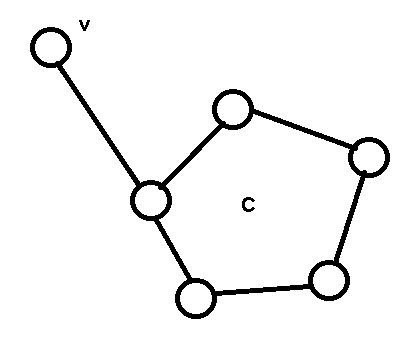
\includegraphics[width=0.3\textwidth]{./pics/graph3.png}

   \item[2.10] \emph{$(\star)$ Αν το γράφημα $G$ είναι Χαμιλτονιανό και $S\subseteq V(G)$, τότε το πλήθος των συνεκτικών συνιστωσών του $G\backslash S$ είναι το πολύ $|S|$.}

Έστω ότι το πλήθος των συνεκτικών συνιστωσών $c$ μπορεί να είναι μεγαλύτερο του $|S|$. Για κάθε συνεκτική συνιστώσα του $G\backslash S$,
οι ακμές που βγαίνουν στο αρχικό γράφημα από τις κορυφές της συνδέονται μόνο με το $S$. Για να υπάρχει κύκλος Hamilton, 
πρέπει να υπάρχουν τουλάχιστον 2 τέτοιες ακμές για κάθε συνιστώσα στον κύκλο Hamilton (σε διαφορετική περίπτωση θα είχαμε
γέφυρα). Σε κάθε ακμή από κάποια συνιστώσα του $G\backslash S$ προς το $S$ αντιστοιχεί και μια κορυφή του $S$ και επειδή στον κύκλο Hamilton όλες οι κορυφές έχουν βαθμό 2, κάθε κορυφή μπορεί να
αντιστοιχεί σε το πολύ 2 συνεκτικές συνιστώσες. Αυτό σημαίνει ότι $|S|\geq \frac{2\cdot c}{2} >  |S|$, άτοπο. Άρα ισχύει το ζητούμενο.


   \item[2.11] \emph{$(\star)$ Ένα τριγωνοποιημένο επίπεδο γράφημα έχει
               χρωματικό αριθμό 3 αν και μόνο αν είναι γράφημα Euler.}

   Θα θεωρήσουμε ότι το γράφημα περιέχει τουλάχιστον 3 κορυφές αφού
   διαφορετικά η πρόταση είναι τετριμμένη.

   Δείχνουμε τις δύο κατευθύνσεις της εκφώνησης ως εξής:

   \begin{itemize}
      \item[$(\Rightarrow)$]
         Έστω (προς απαγωγή σε άτοπο) ότι το $G$ (με $n(G) \geq 3$)
         τριγωνοποιημένο επίπεδο γράφημα το οποίο είναι 3-χρωματίσιμο
         αλλά \emph{δεν} είναι γράφημα Euler.

         Το $G$ θα πρέπει να περιέχει τουλάχιστον μία κορυφή περιττού
         βαθμού, έστω $u \in V(G)$. Η $u$ δεν μπορεί να έχει βαθμό 1
         γιατί διαφορετικά θα βρίσκεται στο σύνορο μίας μόνο
         όψης $f$ η οποία όμως θα πρέπει να έχει στο σύνορό της τουλάχιστον
         άλλες 2 κορυφές. Έστω $v, w$ αυτές οι κορυφές και χωρίς βλάβη της
         γενικότητας έστω $v$ η γειτονική της $u$. Τότε όμως μπορούμε
         να προσθέσουμε την ακμή $\{w, u\}$ και το γράφημα να παραμείνει
         επίπεδο. Αυτό είναι άτοπο γιατί το γράφημα είναι τριγωνοποιημένο,
         δηλαδή η προσθήκη μιας ακμής δεν θα έπρεπε να είναι εφικτή.

         Συνεπώς $d(u) \geq 3$. Έστω $[v_0, v_1, \ldots, v_{k-1}]$
         οι γειτονικές
         κορυφές τις $u$ σε ορολογιακή διάταξη όπως εμφανίζονται στην
         επίπεδη εμβάπτιση του $G$. Αφού το γράφημα είναι τριγωνοποιημένο
         θα πρέπει να υπάρχουν οι ακμές $\{v_i, v_{(i+1) \mod k}\}$ για κάθε
         $i = 0, \ldots, k-1$.

         Άρα η γειτονιά της $u$ ενάγει περιττό κύκλο και αυτό σημαίνει
         ότι χρειάζονται τουλάχιστον 4 χρώματα για το χρωματισμό
         της $u$ και της γειτονιάς της. Άτοπο.

      \item[$(\Leftarrow)$]
         Έστω το ελάχιστο (ως προς πλήθος κορυφών) τριγωνοποιημένο επίπεδο
         γράφημα $G$ το οποίο είναι γράφημα Euler αλλά \emph{δεν} είναι
         3-χρωματίσιμο.% Mπορούμε να υποθέσουμε ότι $n(G) > 3$.

         Το $G$, ως επίπεδο, έχει $\delta(G) \leq 5$. Επειδή όμως είναι
         Euler θα πρέπει ο ελάχιστος βαθμός είτε να είναι 2 είτε 4 (δεν
         μπορεί να είναι $\delta(G) = 0$ γιατί τότε δεν θα ήταν συνεκτικό
         άρα ούτε τρινωνοποιημένο).

         \begin{itemize}
            \item $\delta(G) = 2$.

            Έστω $u$ κορυφή με $d(u) = 2$ και $x, y$ οι γείτονές της.
            Λόγω τριγωνοποίησης έχουμε $e = \{x, y\} \in E(G)$. Όμως
            τώρα η $x$ και η $y$ δεν γίνεται να έχουν άλλους γείτονες
            γιατί λόγω τριγωνοποίησης, η $u$ θα έπρεπε να συνδέεται
            με τουλάχιστον ένα γείτονα της $x$ και της $y$.

            Άρα $G = K_3$ που είναι άτοπο γιατί αυτό είναι 3-χρωματίσιμο.

            \item $\delta(G) = 4$.

            Έστω $u \in V(G)$ με $d(u) = 4$ και $N(u) = \{ v, x, y, w \}$
            όπως φαίνεται στο Σχήμα \ref{fig2.11.1}.

            \begin{figure}
               \centering
               \begin{subfigure}[b]{0.3\textwidth}
                  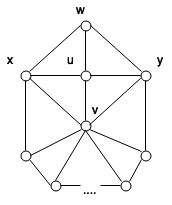
\includegraphics[width=\textwidth]{./pics/fig1.png}
                  \caption{$G$}
                  \label{fig2.11.1}
               \end{subfigure}
               ~
               \begin{subfigure}[b]{0.3\textwidth}
                  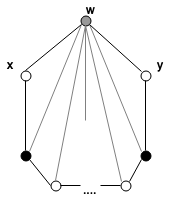
\includegraphics[width=\textwidth]{./pics/fig2.png}
                  \caption{$H$ κι ένας 3-χρωματισμός του}
                  \label{fig2.11.2}
               \end{subfigure}
               ~
               \begin{subfigure}[b]{0.3\textwidth}
                  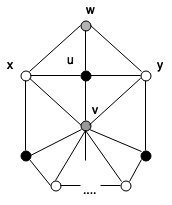
\includegraphics[width=\textwidth]{./pics/fig3.png}
                  \caption{$G$ και ένας 3-χρωματισμός του}
                  \label{fig2.11.3}
               \end{subfigure}
               \caption{Γραφήματα άσκησης 2.11 τα οποία περιέχονται
               ως υπογραφήματα στα $G, H$ και $G$ αντίστοιχα}  
               \label{fig2.11.4}
            \end{figure}

            Λόγω τριγωνοποίησης, οι κορυφές $w, x, v, y$ θα πρέπει να
            σχηματίζουν κύκλο. Ας θεωρήσουμε τώρα τις γειτονικές κορυφές
            της $v$ και στο υπόλοιπο γράφημα. Αυτές θα πρέπει να είναι
            περιττές σε πλήθος αφού ο βαθμός της $v$ πρέπει να είναι
            άρτιος.
            Λόγω τριγωνοποίησης, θα πρέπει
            κι αυτές να σχηματίζουν κύκλο μαζί με τις
            κορυφές $x, y, w$. Επίσης, οι όψεις στων οποίων το περιθώριο
            βρίσκεται η $v$ δεν θα πρέπει να περιέχουν άλλες κορυφές.

            Μετασχηματίζουμε τώρα το $G$ σε ένα γράφημα $H$ όπως φαίνεται
            στο Σχήμα $\ref{fig2.11.2}$ αφαιρώντας τις $u, v$ και τοποθετώντας
            ακμές μεταξύ της $w$ και των γειτόνων της $v$.

            Το $H$ παραμένει επίπεδο και τριγωνοποιημένο καθώς και γράφημα
            Euler (οι βαθμοί των $x, y$ μειώθηκαν κατα 2 και της $w$ μειώθηκε
            κατα 1 και ταυτόχρονα αυξήθηκε κατα περιττό αριθμό, άρα συνολικά
            αυξήθηκε κατα ένα άρτιο αριθμό).

            Άρα το $H$ ώς γράφημα με λιγότερες κορυφές από το $G$,
            θα πρέπει να είναι 3-χρωματίσιμο. Έστω ότι σε αυτό τον
            3-χρωματισμό η $x$ είναι άσπρη και η $w$ γκρί. Τότε
            ο χρωματισμός των υπόλοιπων κορυφών που φαίνονται στο
            Σχήμα $\ref{fig2.11.2}$ προκύπτει ντετερμινιστικά λόγω
            των ακμών που υπάρχουν.

            Παρατηρούμε ότι επειδή η $v$ είχε περιττό πλήθος γειτόνων και
            το μονοπάτι από $x$ στο $y$ πάνω στον κύκλο περιέχει εναλλαγές
            χρωμάτων, το $y$ θα πρέπει να είναι κι αυτό άσπρο.

            Μπορούμε τώρα λοιπόν να προσαρμόσουμε αυτό τον 3-χρωματισμό
            του $H$ στο $G$ βάφοντας την $u$ μαύρη και την $v$ γκρί. Αυτό
            δημιουργεί έναν έγκυρο 3-χρωματισμό για το $G$ το οποίο
            είναι άτοπο.
      \end{itemize}
      Συνεπώς αφού δεν υπάρχει ελάχιστο αντιπαράδειγμα θα πρέπει ένα
      τριγωνοποιημένο επίπεδο γράφημα Euler να είναι 3-χρωματίσιμο.
   \end{itemize}
\end{enumerate}

\section{Επίπεδα γραφήματα}
\section{Τέλεια γραφήματα}
\begin{enumerate}
	\item[4.3] \emph{$(\star)$ Δείξτε ότι για κάθε θετικό ακέραιο $k$ ισχύει ότι ένα γράφημα $G$ είναι τέλειο αν και μόνο αν το $G^{(k)}$ είναι τέλειο.}

Το $G^{(k)}$ είναι ουσιαστικά $k$ αντίγραφα του $G$, με επιπλέον ακμές ανάμεσα σε κάθε δύο κορυφές που βρίσκονται σε διαφορετικά αντίγραφα του $G$.
Από την ισχυρή εικασία των τέλειων γραφημάτων, αν το γράφημα $G$ δεν είναι τέλειο θα έχει περιττή τρύπα μεγέθους τουλάχιστον $5$. Άρα προφανώς και το $G^{(k)}$ θα έχει περιττή τρύπα μεγέθους τουλάχιστον
$5$, αφού περιέχει αντίγραφα του $G$ και κατά την ένωση προστίθενται ακμές μόνο μεταξύ διαφορετικών αντιγράφων του $G$. Άρα ούτε το $G^{(k)}$ θα είναι τέλειο.
Αντίστροφα, έστω ότι το $G^{(k)}$ δεν είναι τέλειο, δηλαδή έχει περιττή τρύπα μεγέθους τουλάχιστον $5$. Αν αυτή περιέχεται στο εσωτερικό ενός αντιγράφου του $G$, τότε περιέχεται και στο $G$ και άρα ούτε
το $G$ είναι τέλειο. Σε διαφορετική περίπτωση, αν οι κορυφές της τρύπας ανήκουν σε τουλάχιστον τρία διαφορετικά αντίγραφα του $G$, τότε θα σχηματίζεται τρίγωνο, το οποίο είναι άτοπο, αφού έχουμε τρύπα
μεγέθους τουλάχιστον $5$.
Η μόνη περίπτωση που μένει είναι οι κορυφές της τρύπας να ανήκουν σε ακριβώς δύο αντίγραφα του $G$, το οποίο είναι και αυτό άτοπο: Κάθε αντίγραφο μπορεί να περιέχει το πολύ δύο κορυφές της τρύπας, γιατί
διαφορετικά θα υπήρχε κορυφή με τρεις γείτονες στην τρύπα. Άρα η μόνη περίπτωση που μπορούμε να έχουμε τρύπα μεγέθους τουλάχιστον $5$ είναι αν αυτή υπάρχει στο $G$, δηλαδή ούτε το $G$ είναι τέλειο.

\end{enumerate}

\section{Μερικές διατάξεις}
\begin{enumerate}
	\item[5.5] \emph{$(\star)$ Δείξτε ότι για κάθε $k$, η κλάση των γραφημάτων με $vc(G)\leq k$ είναι καλώς μερικώς διατεταγμένη ως προς υπογραφήματα.}

Θα υποθέσουμε το αντίθετο, δηλαδή ότι υπάρχει άπειρη αντιαλυσίδα γραφημάτων με $vc(G)\leq k$, κανένα ζευγάρι από τα οποία δεν είναι υπογράφημα του άλλου. Τότε προφανώς
θα υπάρχει $k$, για το οποίο υπάρχει άπειρη αντιαλυσίδα με $vc(G)=k$. Έστω $S$ το σύνολο της κάλυψης ($|S|=k$) και $T=V(G) \backslash S$.
Επίσης επειδή οι διαφορετικοί συνδυασμοί ακμών μεταξύ των κορυφών του $S$ είναι $2^{{k\choose 2}}$, 
δηλαδή πεπερασμένοι, θα υπάρχει ένας από αυτούς, τον οποίο αν σταθεροποιήσουμε θα υπάρχει άπειρη αντιαλυσίδα. 
 Κάθε στοιχείο του $T$ συνδέεται με ένα υποσύνολο των στοιχείων
του $S$. Διαμερίζουμε το σύνολο $T$ με βάση με ποιο υποσύνολο του $S$ είναι συνδεδεμένο με ακμή. Αυτό διαμερίζει το $T$ σε $2^k-1$ σύνολα. Θα αναπαραστήσουμε τα πλήθη αυτών των συνόλων με ένα
σημείο στο $\mathbb{N}^{2^k-1}$. Συγκεκριμένα, η $i$-οστή συντεταγμένη αυτού του σημείου ισούται με το πλήθος των κόμβων που βρίσκονται στο $i$-οστό σύνολο της διαμέρισης. Αν όλες οι συντεταγμένες ενός 
σημείου είναι μικρότερες ή ίσες από αυτές ενός άλλου σημείου, τότε είναι εμφανές ότι το πρώτο γράφημα είναι υπογράφημα του δεύτερου. Αν ορίσουμε λοιπόν τη σχέση μερικής διάταξης
$(x_1,x_2,...,x_m) \leq (y_1,y_2,...,y_m) \Leftrightarrow \forall i\in [1,m] x_i \leq y_i$. Θα αποδείξουμε ότι δεν υπάρχει άπειρη αντιαλυσίδα ως προς αυτή τη σχέση, άρα η αρχική μας υπόθεση είναι άτοπη.

Για να το αποδείξουμε αυτό για κάθε διάσταση, θεωρούμε την ελάχιστη διάσταση $d$ για την οποία υπάρχει άπειρη αντιαλυσίδα. Δεν μπορεί να είναι $d=1$ αφού όλοι οι φυσικοί είναι συγκρίσιμοι μεταξύ τους. 
Έστω τώρα ότι $d>1$. Θεωρούμε ένα στοιχείο $(x_1,x_2,...,x_d)$ της αντιαλυσίδας. Για κάθε άλλο στοιχείο $(y_1,y_2,...,y_d)$, θα πρέπει να υπάρχει $i\in [1,d]$ έτσι ώστε $y_i<x_i$, διότι αλλιώς αυτά
τα δύο στοιχεία θα είναι συγκρίσιμα. Αφού η αντιαλυσίδα είναι άπειρη και οι διαστάσεις πεπερασμένες, θα υπάρχει $i\in [1,d]$ έτσι ώστε να υπάρχει άπειρη αντιαλυσίδα με $y_i<x_i$ για κάθε στοιχείο της
αλυσίδας.
Επειδή όμως το $x_i$ είναι πεπερασμένο, υπάρχουν πεπερασμένα τέτοια διαφορετικά $y_i$, και άρα θα υπάρχει άπειρη αντιαλυσίδα έτσι ώστε όλα τα στοιχεία της να έχουν την ίδια $i$-οστή συντεταγμένη.
Τότε, όμως, αν αγνοήσουμε την $i$-οστή συντεταγμένη, έχουμε βρει μια άπειρη αντιαλυσίδα στις $d-1$ διαστάσεις. Αυτό είναι άτοπο, αφού έχουμε θεωρήσει το $d$ ως ελάχιστο αντιπαράδειγμα.


	\item[5.6] \emph{$(\star)$ Δείξτε ότι, για κάθε $k$, κάθε γράφημα στο σύνολο παρεμπόδισης ελασσόνων της κλάσης $C_k=\{G|\vc(G)\leq k\}$ έχει $O(k^2)$ κορυφές.}

Αρκεί να δείξουμε ότι κάθε γράφημα $G$ με $\vc(G)>k$ έχει ως ελάσσον ένα $H$ με $\vc(H)>k$ και $O(k^2)$ κορυφές. Στην πραγματικότητα θα δείξουμε ότι περιέχει σαν εναγόμενο υπογράφημα ένα τέτοιο γράφημα.
Έστω γράφημα $G$ με $\vc(G)>k$ και έστω $S$ το σύνολο που πραγματοποιεί την κάλυψη ($|S|=\vc(G)$). Επίσης θεωρούμε τη διαμέριση του $S$ σε δύο σύνολα $A$ και $B$, ώστε οι κορυφές του $A$ να 
είναι αυτές που έχουν τουλάχιστον
$k+1$ ακμές προς το $V(G)\backslash A$, και $B$ οι υπόλοιπες. Διακρίνουμε τρεις περιπτώσεις: 
\begin{itemize}

\item{a.}
Αν έχουμε ότι $|A| \geq k+1$, τότε διαγράφουμε οποιεσδήποτε $|A|-(k+1)$ κορυφές του $A$, όλες τις κορυφές του $B$, καθώς και όλες τις κορυφές του 
$V(G)\backslash S$ που έγιναν απομονωμένες. Στη συνέχεια, για κάθε κορυφή στο $A$, μαρκάρουμε οποιουσδήποτε $k+1$ γείτονες στο $V(G)\backslash S$. Αν κάποια κορυφή του $V(G)\backslash S$ δεν έχει
μαρκαριστεί, διαγράφεται και αυτή. Στο γράφημα $G'$ 
που έχει προκύψει, έχουμε κάλυψη με $k+1$ κορυφές χρησιμοποιώντας όλα τα στοιχεία του $A$. Αν δεν χρησιμοποιήσουμε έστω και ένα στοιχείο του $A$,
θα πρέπει να είναι στο σύνολο της κάλυψης οι $k+1$ γείτονες που έχει στο $V(G)\backslash S$. Άρα έχουμε $\vc(G')>k$.

\item{b.}
Αν $|S|=\Theta(k)$, τότε μαρκάρουμε όλους τους γείτονες των κορυφών του $B$ στο $V(G)\backslash S$, αλλά και οποιουσδήποτε $k+1$ γείτονες στο $V(G)\backslash S$, για κάθε μία κορυφή του $A$.
Διαγράφουμε όλες τις κορυφές του $V(G)\backslash S$ που δεν μαρκάραμε.
Στο γράφημα $G'$ που προέκυψε, κάθε κορυφή του $S$ πλέον έχει $O(k)$ γείτονες στο $V(G)\backslash S$, άρα συνολικά έχουμε $O(k^2)$ κορυφές. Επίσης, από το ίδιο επιχείρημα που χρησιμοποιήσαμε στην
περίπτωση 1, όλες οι κορυφές του $A$ είναι στο σύνολο κάλυψης. Έστω τώρα ότι υπάρχει κάλυψη μικρότερη από $|S|$. Αυτό θα σήμαινε ότι το σύνολο $B$ θα μπορούσαμε στην αρχική κάλυψη να το
αντικαταστήσουμε με ένα μικρότερο $B'$. Αυτό γιατί καμία από τις κορυφές που σβήστηκαν από το $G$ δεν είχαν ακμή προς το $B$, συνεπώς οι ακμές τους ικανοποιούνταν από το $A$. Αυτό είναι όμως άτοπο,
άρα $\vc(G')\geq\min(\vc(G),k+1)>k$.

\item{c.}
Σε αυτή την περίπτωση έχουμε $|A|\leq k$ και $|S|=\omega(k)$ (άρα και $|B|=\omega(k)$). Τώρα, όπως και στα προηγούμενα, μαρκάρουμε για κάθε στοιχείο του $A$, οποιουσδήποτε $k+1$ γείτονές του στο
$V(G)\backslash S$. Στη συνέχεια διαλέγουμε οποιεσδήποτε $k+1$ κορυφές από το $B$, μαρκάρουμε όλους τους γείτονες κάθε μίας στο $V(G)\backslash S$ και σβήνουμε όλες τις υπόλοιπες κορυφές του $B$,
φτιάχνοντας έτσι ένα νέο σύνολο $B'$.
Τέλος, σβήνουμε όλες τις κορυφές του $V(G)\backslash S$ που δεν έχουν μαρκαριστεί ή είναι απομονωμένες. Είναι προφανές ότι έχουμε καταλήξει σε ένα γράφημα $G'$
με $O(k^2)$ κορυφές. Όλα τα στοιχεία του $A$ θα ανήκουν
στο σύνολο κάλυψης, και τα υπόλοιπα που θα ανήκουν στο σύνολο κάλυψης δεν μπορεί να είναι λιγότερα από $B'$, καθώς καμία από τις κορυφές του $V(G)\backslash S$ που έχουν σβηστεί δεν έχει ακμή
προς το $B'$. Συνεπώς έχουμε $\vc(G')\geq |A| + |B'| > k$.

\end{itemize}
Σε κάθε περίπτωση, λοιπόν, ένα γράφημα $G$ με $\vc(G)>k$ έχει εναγόμενο υπογράφημα $H$ με $\vc(H)>k$ και $O(k^2)$ κορυφές, και άρα το ζητούμενο έχει αποδειχθεί.


	\item[5.7] \emph{$(\star)$ Έστω $\mathcal{U}_r$ το σύνολο παρεμπόδισης ελασσόνων για την κλάση γραφημάτων με προσανατολισμένο γένος το πολύ $r$. Δείξτε ότι δεν υπάρχει πολυώνυμο $p$ τέτοιο ώστε
$|\mathcal{U}_r|\leq p(r)$.}

Θα δείξουμε ότι το μέγεθος του συνόλου παρεμπόδισης ελασσόνων αυξάνεται τουλάχιστον εκθετικά με το $r$. Θα χρησιμοποιήσουμε το Λήμμα που λέει ότι αν $G_1, ..., G_k$ οι δισυνεκτικές συνιστώσες
ενός γραφήματος $G$, τότε $\gamma (G) = \sum_{i=1}^k \gamma(G_i)$. Αν κάθε δισυνεκτική συνιστώσα ταυτίζεται με το $K_5$, τότε, εφόσον $\gamma (K_5)=1$, έχουμε $\gamma (G) = k$.

Θεωρούμε την οικογένεια μη ετικετωμένων δένδρων με $r+1$ κόμβους. Για κάθε δέντρο, δημιουργούμε ένα γράφημα ως εξής: 
Στη θέση κάθε κόμβου τοποθετούμε ένα αντίγραφο του $K_5$, και για κάθε ακμή στο δέντρο ταυτίζουμε δύο κόμβους των $K_5$ που αντιστοιχούν
στα άκρα της ακμής. Το γράφημα που έχουμε δημιουργήσει έχει γένος ακριβώς $r+1$. Επίσης, όλα τα γραφήματα που έχουμε δημιουργήσει είναι διαφορετικά μεταξύ τους και ανήκουν στο $\mathcal{U}_r$:
Έστω ότι κάποιο δεν ανήκε. Αυτό σημαίνει ότι έχει σαν ελάσσον ένα γράφημα με γένος $r+1$. Αυτό όμως δεν ισχύει, διότι σβήνοντας ή συνθλίβοντας μια ακμή από κάποιο 
$K_5$, η δισυνεκτική συνιστώσα που αντιστοιχεί
σε αυτό έχει πλέον γένος $0$, άρα το συνολικό γένος είναι $r$. Ομοίως, σβήνοντας μια κορυφή, μία ή περισσότερες δισυνεκτικές συνιστώσες θα αποκτήσουν γένος $0$, άρα το συνολικό γένος θα είναι $\leq r$,
άτοπο. 
\newline
Επειδή γνωρίζουμε ότι το πλήθος των μη ετικετωμένων δένδρων αυξάνεται εκθετικά συναρτήσει του πλήθους των κόμβων του ($r+1$), παίρνουμε το ζητούμενο.

\end{enumerate}


\section{$k$-δέντρα}

\begin{enumerate}
   \item[6.2] \emph{Καλούμε μερικό $k$-δέντρο κάθε υπογράφημα $k$-δέντρου.
   Δείξτε ότι το $K_{r,r}$ είναι μερικό $r$-δέντρο αλλά δεν είναι μερικό
   $(k-1)$-δέντρο.}

   Το $K_{r,r}$ είναι μερικό $k$-δέντρο αφού μπορούμε να το παράγουμε
   ως εξής:

   Ξεκινάμε με το $K_{r+1}$ και διαλέγουμε μία κορυφή του την οποία
   αναθέτουμε στο σύνολο $X$ και τις υπόλοιπες τις αναθέτουμε στο σύνολο
   $Y$. Το $Y$ είναι μια $r$-κλίκα επομένως μπορούμε να τοποθετήσουμε
   $r-1$ νέες κορυφές στο $X$ κάθε μία από τις οποίες τις συνδέουμε
   με όλες τις κορυφές του $Y$.

   Τώρα αφαιρούμε όλες τις ακμές μεταξύ κορυφών του $Y$ και αυτό
   που μένει είναι το $K_{r,r}$.

   Έστω τώρα ότι το $K_{r,r}$ ήταν μερικό $(r-1)$-δέντρο. Τότε θα πρέπει
   να περιέχει μια κορυφή $u$ με $d(u) < r$ (η τελευταία κορυφή που προσθέσαμε
   κατα της κατασκευή του $(r-1)$-δέντρου είχε βαθμό $r-1$). Αυτό όμως είναι
   άτοπο γιατί όλες οι κορυφές του $K_{r,r}$ έχουν βαθμό ίσο με $r$.


	\item[6.4] \emph{$(\star)$ Αν ένα χορδικό γράφημα είναι επίπεδο, τότε θα είναι και μερικό $3$-δέντρο.}

Γνωρίζουμε ότι ένα γράφημα έχει δενδροπλάτος $k$ αν και μόνο αν η μεγαλύτερη κλίκα της χορδικής κλειστότητάς του είναι $k+1$. Εφόσον έχουμε χορδικό γράφημα, αυτό ταυτίζεται με την χορδική του κλειστότητα,
και μάλιστα εφόσον είναι επίπεδο, δεν μπορεί να έχει κλίκα μεγαλύτερη του $4$. Αυτό σημαίνει ότι το δενδροπλάτος του είναι το πολύ $3$, δηλαδή θα είναι μερικό $3$-δέντρο.

	\item[6.5] \emph{Δείξτε ότι ο τρισδιάστατος υπερκύβος είναι μερικό $3$-δέντρο.}

Στο παρακάτω σχήμα απεικονίζεται μία χορδική κλειστότητα του τρισδιάστατου κύβου, η οποία εύκολα φαίνεται ότι είναι επίπεδο γράφημα. Συνεπώς, από την άσκηση $6.4$, ο τρισδιάστατος υπερκύβος είναι μερικό 
$3$-δέντρο.
\newline
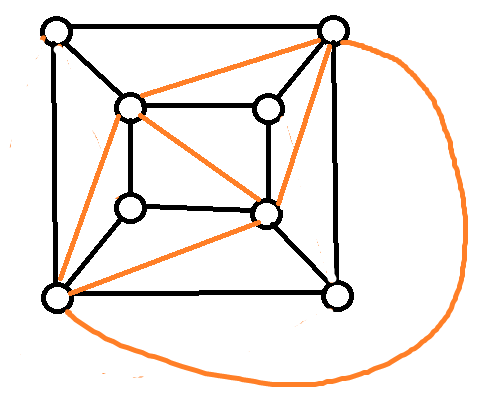
\includegraphics[width=0.3\textwidth]{./pics/graph1.png}

   \item[6.6] \emph{$(\star)$ Τα γραφήματα τομών των υποδέντρων
   δέντρων είναι τα γραφήματα χωρίς εναγόμενους κύκλους μήκους μεγαλύτερου
   του 3.}

   Το γράφημα τομών υποδέντρων δέντρων για ένα δέντρο $T$ είναι ένα
   γράφημα $G$ με κορυφές κάποιο υποσύνολο του συνόλου των υποδέντρων του
   $T$. Ακμή
   μεταξύ δύο υποδέντρων υπάρχει αν αυτά έχουν μη κενή τομή.
   Πιο τυπικά: $V(G) \subseteq \{ R\ |\ R \subseteq T \text{ και }
   R \text{ είναι δέντρο } \}, E(G) = \{ \{T_1, T_2\}\ |\ T_1, T_2 \in V(G)\
   \text{ και } T_1 \cap T_2 \neq \emptyset \}$.

   \begin{lm}
      \label{lm6.6.1}
      Έστω $T_1, T_2 \subseteq T$ υποδέντρα του $T$ με $T_1 \cap T_2 \neq
      \emptyset$ δύο κορυφές $u \in T_1, v \in T_2$. Τότε υπάρχει μονοπάτι
      από την $u$ στην $v$ που χρησιμοποιεί μόνο κορυφές από το
      $V(T_1 \cup T_2)$.
   \end{lm}
   \begin{proof}
      Έστω $w \in V(T_1 \cap T_2)$. Επειδή το $T_1$ είναι συνεκτικό (ως δέντρο)
      υπάρχει μονοπάτι $P_1$ από την $u$ στην $w$ που διέρχεται μέσα
      από το $T_1$. Αντίστοιχα υπάρχει $P_2$ από την $w$ στην $v$
      που να διέρχεται μέσα από το $P_2$.

      Οι μόνες κοινές κορυφές που έχουν τα $P_1, P_2$ μπορεί να είναι
      κάποιο επίθεμα του $P_1$ με κάποιο πρόθεμα του $P_2$.
      Γιατί διαφορετικά, αν $P_2 = [w, x_1, \ldots, x_k, \ldots]$
      όπου η $x_k$ είναι η πρώτη κορυφή μετά την $w$ στο μονοπάτι
      $P_2$ που να εμφανίζεται στο $P_1$ τότε μπορεί να δημιουργηθεί
      ο κύκλος: $x_kP_1 \cup P_2x_k$ \footnote{Με το συμβολισμό
      $uP$ εννοούμε το υπομονοπάτι του $P$ που ξεκινάει από την $u$
      και συνεχίζει μέχρι το τέλος του $P$. Αντίστοιχα και για το $Pu$
      (βλ. παράγραφος 1.3 του βιβλίου του Diestel).}.

      Έστω λοιπόν ότι $P_1 = P_1' \cup P, P_2 = P \cup P_2'$.
      Τότε το μονοπάτι $R = P_1' \cup P_2'$ είναι το μονοπάτι
      από την $u$ στη $v$ που αναζητούμε.
   \end{proof}

   Ας υποθέσουμε ότι το $G$ έχει εναγόμενο κύκλο $C = [T_1, \ldots T_{k},
   T_1]$ μήκους τουλάχιστον $k >= 4$. Αρχικά θα δείξουμε ότι για κάθε
   $i \leq k-1$ και κάθε δύο κορυφές $u \in T_1, v \in T_i$ υπάρχει
   μονοπάτι από την $u$ στην $v$ διαμέσου του δέντρου $T_1 \cup \ldots \cup
   T_i$. Αυτό γίνεται εύκολα με επαγωγή αφού αν υποθέσουμε
   ότι αυτό ισχύει για το ζεύγος κορυφών $u \in T_1, w \in T_{i-1}$
   μπορούμε να χρησιμοποιήσουμε το Λήμμα \ref{lm6.6.1} με τα δέντρα
   $T_1 \cup \ldots \cup T_{i-1}$ και $T_i$ (έχουν μή κενή τομή αφού
   $T_{i-1} \cap T_i \neq \emptyset$).

   Για το $T_k$ τώρα ξέρουμε ότι $T_1 \cap T_k \neq \emptyset$
   και $T_{k-1} \cap T_{k} \neq \emptyset$. Έστω δύο κορυφές
   $u \in T_1 \cap T_{k}, v \in T_{k-1} \cap T_k$. Οι κορυφές αυτές
   δεν θα πρέπει να ανήκουν σε κανένα από τα $T_i$ για $2 \leq i \leq k-2$
   διαφορετικά θα υπήρχε χορδή στον κύκλο $C$. Παίρνουμε λοιπόν
   το μονοπάτι $P$ που πάει από την $u$ στην $v$ και διέρχεται από
   το δέντρο $T_1 \cup \ldots \cup T_{k-1}$.

   Εφαρμόζοντας το Λήμμα \ref{lm6.6.1} δύο φορές με τα δέντρα
   $T_1, T_k, T_{k-1}$ παίρνουμε ένα μονοπάτι $P'$ από την $u$
   στη $v$ που διέρχεται από το δέντρο $T_1 \cup T_k \cup T_{k-1}$.
   Επειδή όμως το $T$ είναι δέντρο, το μονοπάτι μεταξύ $u$ και
   $v$ θα πρέπει να είναι μοναδικό άρα $P \equiv P'$.

   Εδώ καταλήγουμε σε άτοπο γιατί $T_1 \cap T_{k-1} = \emptyset$ κι έτσι
   υπάρχει κορυφή $w \in P'$ που να βρίσκεται στο $T_k \backslash T_1
   \backslash T_{k-1}$, κι επειδή $P \equiv P'$,
   $w \in P$, δηλαδή το $T_k$ έχει κοινή κορυφή με κάποιο από τα
   $T_i$ για $i = 2, \ldots, k-2$. Άτοπο γιατί τότε θα υπήρχε χορδή
   στον $C$.
\end{enumerate}

\section{Άπειρα γραφήματα}

\begin{enumerate}
   \item[7.1] \emph{Έστω $r \in \mathbb{Z}_{\geq 1}, t \in (0, 2)$
   και $C_r = \{ \mathbf{p} = \{x_1, \ldots, x_r\} \in \mathbb{R}^r\ |\ 
   x_1^2 + \ldots x_r^2 = 1 \}$. Έστω επίσης το άπειρο γράφημα
   $G_r^t$ που έχει ως σύνολο κορυφών το $C_r$ και όπου δύο σημεία
   συνδέονται με μία ακμή ανν η Ευκλείδεια απόστασή τους είναι
   ακριβώς $t$. Έστω τέλος το σύνολο:}

   \[ H_r = \{ t\ |\ G_r^t \text{ έχει άπειρες συνεκτικές συνιστώσες} \} \]

   \emph{Δείξτε ότι $|H_2| = \aleph_0$. Ισχύει το ίδιο για $r \geq 3$;}
   \newline

   Για $r=2$ το $G_r^t$ είναι κύκλος ακτίνας 1 στο επίπεδο. Έστω
   2 σημεία $P, P'$ πάνω στον κύκλο που απέχουν ευκλείδια απόσταση $t$
   όπως φαίνεται στο παρακάτω σχήμα.

   \begin{center}
      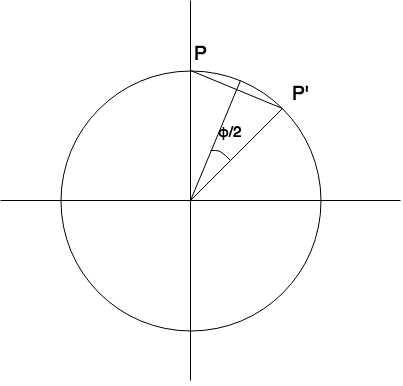
\includegraphics[width=0.4\textwidth]{./pics/geom.png}
   \end{center}

   Για το μήκος του τόξου $\stackrel\frown{PP'}$ έχουμε
   $\sin \left( \frac{\phi}{2} \right) = \frac{t}{2}
   \Leftrightarrow \phi = 2 \arcsin \left( \frac{t}{2} \right)$
   (η γωνία $\phi$ μετριέται σε ακτίνια και έτσι ισούται με το
   μήκος του ζητούμενου τόξου).

   Αν ισχύει $\kappa \cdot \phi = \lambda \cdot 2\pi$ 
   για $\kappa, \lambda \in \mathbb{Z}_+$ τότε υπάρχει
   κύκλος πεπερασμένου μήκους $\kappa$ στο $G_r^t$ που να ξεκινάει από το
   $P$, να διασχίζει τον κύκλο $\lambda$ φορές (χωρίς όμως να περνάει
   από το ίδιο σημείο δύο φορές) και να καταλήγει πάλι στο $P$.

   Δηλαδή αν $\frac{\phi}{2\pi} \in \mathbb{Q} \Leftrightarrow
   \frac{1}{\pi} \arcsin \left( \frac{t}{2} \right) \in \mathbb{Q}$
   τότε το $P$ (για ένα αυθαίρετα επιλεγμένο $P$) βρίσκεται σε συνεκτική
   συνιστώσα που είναι κύκλος πεπερασμένου μήκους. Αφού αυτό
   ισχύει για κάθε $P$, έχουμε ότι οι συνεκτικές συνιστώσεις του $G_r^t$
   αποτελούνται από πεπερασμένους κύκλους και συνεπώς θα πρέπει
   να είναι (μη αριθμήσιμα) άπειρες σε πλήθος.

   Συμβολίζουμε με $f(t) = \frac{1}{\pi} \arcsin \left( \frac{t}{2} \right)$
   τη συνάρτηση $f\ :\ (0, 2) \rightarrow (0, 1)$ η οποία είναι
   1-1, επί.
   
   Με βάση αυτό το συμβολισμό έχουμε ότι όταν $f(t) \in \mathbb{Q}$,
   τότε το $G_r^t$ αποτελείται από άπειρες συνεκτικές συνιστώσες
   πεπερασμένου μεγέθους η κάθε μία.

   Από την άλλη, αν $f(t) \in \mathbb{R} \backslash \mathbb{Q}$,
   τότε αν πάρουμε μια κορυφή $u \in V(G_r^t)$, μπορούμε να δημιουργήσουμε
   δύο άπειρα μονοπάτια με αφετηρία τη $u$ (ένα για
   κάθε γείτονα της $u$). Άρα η συνεκτική συνιστώσα στην οποία
   βρίσκεται η $u$ θα πρέπει να περιέχει αριθμήσιμες σε πλήθος κορυφές
   αφού μπορούμε να τις αριθμήσουμε ακολουθώντας τα δύο αυτά μονοπάτια.

   Επειδή όμως το γράφημα έχει μη αριθμήσιμες κορυφές, το πλήθος
   των συνεκτικών του συνιστωσών δεν μπορεί να είναι πεπερασμένο.

   Δείξαμε λοιπόν ότι $H_2 = (0, 2)$\footnote{Αυτό προφανώς αντιβαίνει σε αυτό
   που ζητάει η άσκηση και πιθανώς το λάθος στην απόδειξή μας να οφείλεται
   στο ότι χρησιμοποιήσαμε κάποιο non-standard ορισμό για το τί είναι
   μονοπάτι ή τί είναι συνεκτική συνιστώσα σε άπειρο γράφημα.}

   %Με βάση όσα έχουμε πεί, ισχύει ότι:
   %$H_r = \{ t\ |\ f(t) \in \mathbb{Q} \}$. Στο σύνολο τιμών της $f$
   %υπάρχουν $\aleph_0$ ρητοί αριθμοί, άρα υπάρχει ίδιο πλήθος $t$
   %στο πεδίο ορισμού της για τα οποία $f(t) \in \mathbb{Q}$, άρα
   %πράγματι $|H_r| = \aleph_0$.

   \item[7.2] \emph{Έστω $G_r$ το (άπειρο) γράφημα με $V(G_r) = \mathbb{R}^r$
   και όπου δύο κορυφές ενώνονται αν η μεταξύ τους Ευκλείδεια απόσταση είναι
   1. Δείξτε ότι $3 \leq \chi(G_2) \leq 7$. Βρείτε στη βιβλιογραφία
   τις καλύτερες εκτιμήσεις του $\chi(G_r)$ για $r > 2$.}

   Αρχικά παρατηρούμε ότι αν πάρουμε οποιοδήποτε ισόπλευρο τρίγωνο
   πλευράς 1 στο επίπεδο, αυτό αποτελεί κλίκα 3 κορυφών στο $G_2$ και
   έτσι έχουμε $\chi(G_2) \geq 3$.

   Το κάτω φράγμα μπορεί να βελτιωθεί αν θεωρήσουμε το παρακάτω γράφημα
   (Γράφημα Golomb) το οποίο αποτελείται από ένα τροχό πλευράς 1 και ένα
   ισόπλευρο τρίγωνο πλευράς 1
   τοποθετημένα στο επίπεδο έτσι ώστε τρεις από τις κορυφές του εξαγώνου
   να συνδέονται με τις κορυφές του τριγώνου. Το γράφημα αυτό
   απαιτεί 4 χρώματα για το χρωματισμό του, επομένως $\chi(G_2) \geq 4$.

   \begin{center}
      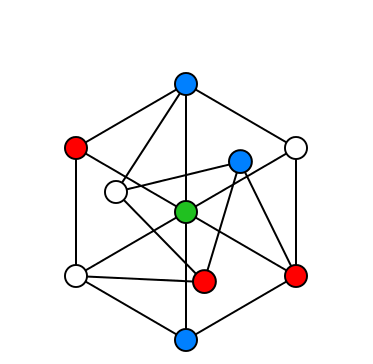
\includegraphics[width=0.3\textwidth]{./pics/golomb.png}
   \end{center}

   Για το άνω φράγμα, παρατηρούμε ότι μπορούμε καλύψουμε το επίπεδο
   με χρωματιστά εξάγωνα διαμέτρου $1 - \epsilon$ όπως φαίνεται
   στο παρακάτω σχήμα:

   \begin{center}
      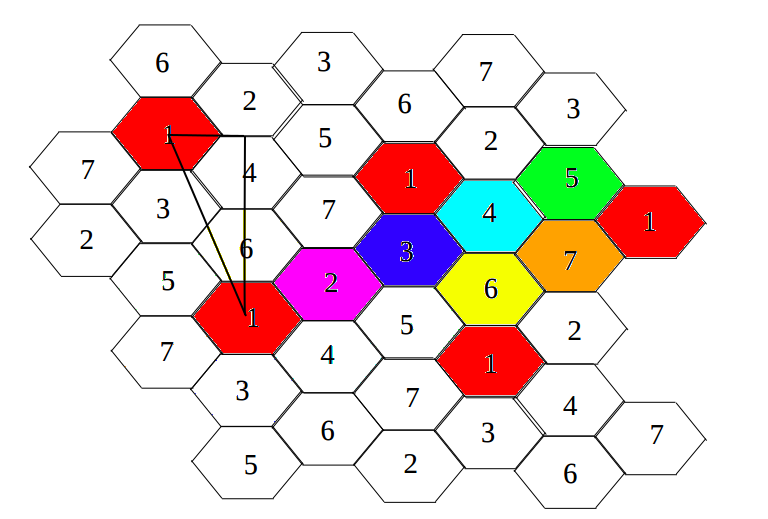
\includegraphics[width=0.5\textwidth]{./pics/grid.png}
   \end{center}

   Ο τρόπος με τον οποίο καλύπτουμε το επίπεδο είναι
   να δημιουργήσουμε διαγώνιες λωρίδες με εφαπτόμενα εξάγωνα τα οποία
   είναι χρωματισμένα με τα χρώματα 1-7 με αυτή τη σειρά και αυτό το
   σχήμα (pattern) να επαναλαμβάνεται άπειρες φορές. Έχοντας λοιπόν
   τοποθετήσει μια τέτοια λωρίδα από εξάγωνο στο επίπεδο, τοποθετούμε
   τις υπόλοιπες από πάνω αριστερά της (και κάτω δεξιά) μετατοπισμένη
   (shifted) κατά δύο θέσεις (βλ. τις θέσεις των εξαγώνων με χρώμα
   1 στο σχήμα).
   
   Ας δούμε τώρα πόση είναι η ελάχιστη Ευκλείδεια απόσταση μεταξύ δύο
   σημείων του επιπέδου με το ίδιο χρώμα. Κατ αρχάς αν αυτά τα σημεία
   βρίσκονται στο ίδιο εξάγωνο δεν γίνεται να έχουν απόσταση 1 γιατί
   η διάμετρος κάθε εξαγώνου είναι $1 - \epsilon < 1$.
   
   Αρκεί λοιπόν να θεωρήσουμε σημεία μεταξύ διαφορετικών εξαγώνων.
   Χωρίς βλάβη της γενικότητας
   θεωρούμε το ένα εξάγωνο με χρώμα 1 και ένα από τα 6 εξάγωνα
   ίδιου χρώματος που βρίσκονται
   πιο κοντά σε αυτό (λόγω συμμετρίας αρκεί να μελετήσουμε την απόσταση
   σε σχέση με ένα από αυτά τα 6 εξάγωνα). Η ελάχιστη απόσταση μεταξύ 2
   σημείων των εξαγώνων αυτών μπορεί να φραχτεί από κάτω από την
   ελάχιστη απόσταση μεταξύ σημείων δύο κύκλων ακτίνας $~\frac{1}{2}$
   με κέντρα τα αντίστοιχα κέντρα των εξαγώνων.

   Δηλαδή αν $R = \frac{1-\epsilon}{2}$
   η ακτίνα των δύο κύκλων και $d$ η απόσταση των δύο κέντρων
   (μπορούμε από το ορθογώνιο τρίγωνο του σχήματος να υπολογίσουμε
   ότι $d \sim \frac{\sqrt{21}}{2}$) τότε η ελάχιστη απόσταση
   δύο σημείων των κύκλων είναι $d - 2R \sim d - 1
   = \frac{\sqrt{21}}{2} - 1 > 1$.

   Συνεπώς ο χρωματισμός που προτείναμε είναι ένας έγκυρος 7-χρωματισμός
   τους επιπέδου κι έτσι $\chi(G_2) \leq 7$.

   \paragraph{Ιστορικά στοιχεία}

   Το πρόβλημα αυτό (για $r = 2$) είναι γνωστό στη βιβλιογραφία
   ως Hadwiger–Nelson problem. Παραμένει μέχρι σήμερα ανοικτό
   και η καλύτερη εκτίμηση που έχουμε είναι $4 \leq \chi(G_4) \leq 7$.
   
   Είναι ενδιαφέρον το γεγονός ότι η λύση του προβλήματος μπορεί
   να εξαρτάται από το ποιά αξιώματα της θεωρίας συνόλων έχουμε
   επιλέξει και συγκεκριμένα από το αν θα συμπεριλάβουμε το αξίωμα
   της επιλογής (βλ. ``Axiom of choice and chromatic number of the plane''
   [Shelah, Soifer, 2003]).

   \paragraph{Γενίκευση για $r > 2$}

   Για τις 3 διστάσεις γνωρίζουμε ότι $6 \leq \chi(G_4) \leq 15$
   [Nechushtan 2002] [Coulson 2002].

   Για μεγαλύτερες διαστάσεις έχουμε μόνο κάτω φράγματα
   καθώς και ένα ασυμπτωτικό φράγμα για μεγάλα $r$:
   $(1,239 + o(1))^r \leq \chi(G_r) \leq (3 + o(1))^r$ από
   τους [Raigorodskii, 2000], [Larman, Rogers, 1972].

   \item[7.3] \emph{$(\star)$ Χρησιμοποιώντας το λήμμα του K\H{o}nig, αποδείξτε
   ότι αν το $G$ είναι γράφημα όπου $|V(G)| = \aleph_0$ και κάθε υπογράφημά
   του είναι 3-χρωματίσιμο, τότε και το $G$ είναι 3-χρωματίσιμο.}

   Έστω $V(G) = \{ 1, 2, \ldots, n, \ldots \}$. Συμβολίζουμε με $G[k]$
   το εναγόμεμο υπογράφημα του $G$ με κορυφές τις $\{1, \ldots, k\}$.

   Δημιουργούμε το εξής δέντρο $T$: Κάθε κόμβος του δέντρου εκτός της ρίζας
   αντιστοιχεί σε ένα έγκυρο 3-χρωματισμό του $G[k]$ για κάποιο $k$.
   Συγκεκριμένα, η ρίζα έχει 3 παιδιά που αντιστοιχούν στους τρεις πιθανούς
   χρωματισμούς του $G[1]$ και αν ένας κόμβος $u \in T$ αντιστοιχεί σε
   3-χρωματισμό
   του $G[k]$, τότε θεωρούμε το γράφημα $G[k+1] \supseteq G[k]$ καθώς και κάθε
   3-χρωματισμό του που συμφωνεί με το χρωματισμό του $G[k]$. Υπάρχουν
   3 τέτοιοι χρωματισμοί (3 επιλογές για το χρώμα της νεας κορυφής).
   και ώς παιδία της $u$ θέτουμε τους έγκυρους από αυτούς
   τους χρωματισμούς.

   Παρατηρούμε ότι ένας κόμβος $u$ βρίσκεται σε απόσταση $r$ από τη ρίζα
   του $T$ αν και μόνο αν το $u$ αντιστοιχεί σε έγκυρο 3-χρωματισμό
   του $G[r]$.

   Για το γράφημα $T$ γνωρίζουμε ότι κάθε κόμβος έχει πεπερασμένο βαθμό
   (το πολύ 4) και ότι έχει άπειρο πλήθος κόμβων γιατί σύμφωνα με την
   προηγούμενη παρατήρηση, αν τo $G[k]$ είναι 3-χρωματίσιμο θα πρέπει
   να υπάρχει τουλάχιστον μια κορυφή $u$ που να αντιστοιχεί στο
   χρωματισμό του. Ξέρουμε όμως ότι όλα τα $G[k]$ για $k \in \mathbb{N}$
   είναι 3-χρωματίσιμα άρα θα πρέπει να υπάρχει τουλάχιστον μια κορυφή
   για κάθε τέτοιο $k$.

   Από το λήμμα του K\H{o}nig έχουμε λοιπόν ότι πρέπει να υπάρχει άπειρο
   μονοπάτι $P$ που να ξεκινάει από τη ρίζα. Το μονοπάτι αυτό ορίζει
   έναν 3-χρωματισμό του $G$ (το χρώμα μιας κορυφής $w \in V(G)$
   είναι το χρώμα που του αναθέτει ο χρωματισμός του $G[w]$ στο μονοπάτι
   $P$). O χρωματισμός αυτός είναι έγκυρος γιατί διαφορετικά, αν υπάρχουν
   κορυφές $u, v \in V(G)$ με $\{u, v\} \in E(G)$ και ίδιο χρώμα, τότε
   ο χρωματισμός του $G[\max(u, v)]$ στο μονοπάτι $P$ δεν θα ήταν έγκυρος.
\end{enumerate}

\section{Κανονικά γραφήματα και Ταιριάσματα}
\begin{enumerate}
   \item[8.1] \emph{$(\star)$ Κάθε διμμερές $k$-κανονικό γράφημα όπου
   $k \geq 1$ έχει τέλειο ταίριασμα.}

   Έστω $X, Y$ τα δύο μέρη του $G$ και έστω $S \subseteq X$. Υποθέτουμε,
   προς απαγωγή σε άτοπο ότι $|N(S)| < |S|$. 

   Έστω $E_S$ το σύνολο των ακμών που προσπίπτουν στο $S$.
   Επειδή το $G$ είναι $k$-κανονικό, έχουμε
   $|E_S| = k \cdot |S|$. Από την άλλη, μετρώντας τις
   ακμές που προσπίπτουν στον $N(G)$ έχουμε μια υπερεκτίμιση
   του $|E_S|$, δηλαδή $k \cdot |N(S)| \geq |E_S| = k \cdot |S|$.
   Αυτό όμως είναι άτοπο γιατί υποθέσαμε $|N(S)| < |S|$.

   Συνεπώς από το Θεώρημα Hall έχουμε ότι υπάρχει ταίριασμα που
   να καλύπτει όλες τις κορυφές του $X$.

   Επειδή όμως το $G$ είναι $k$-κανονικό, μπορούμε να δείξουμε ότι
   $|X|=|Y|$ και συνεπώς το ταίριασμα που βρήκαμε είναι τέλειο.
   Πράγματι, αν μετρήσουμε τις ακμές του γραφήματος με δύο τρόπους,
   πρώτα μετρώντας τις προσκείμενες στο $X$ και εξισώνοντας με
   το πλήθος των ακμών που είναι προσκείμενες στο $Y$ έχουμε
   $k \cdot |X| = k \cdot |Y| \Leftrightarrow |X| = |Y|$.

	\item[8.2] \emph{$(\star\star)$ Δείξτε ότι κάθε συνεκτικό γράφημα με άρτιο αριθμό ακμών μπορεί να προσανατολιστεί έτσι ώστε κάθε κορυφή να έχει άρτιο εξώβαθμο.
Χρησιμοποιώντας αυτό δείξτε ότι κάθε $3$-κανονικό γράφημα με $4k$ κορυφές περιέχει ανεξάρτητο σύνολο με $k$ κορυφές το οποίο αν αφαιρεθεί από το $G$ δημιουργεί γράφημα
του οποίου όλες οι συνεκτικές συνιστώσες είναι μονοκυκλικές}

\begin{proof}
Αρχικά θα αποδείξουμε το πρώτο. Έστω ένας τυχαίος προσανατολισμός των ακμών του γραφήματος. Αυτός διαμερίζει τις κορυφές σε δύο σύνολα, το $A$ που περιέχει τις κορυφές με άρτιο
εξώβαθμο, και το $B$ που περιέχει τις κορυφές με περιττό εξώβαθμο. Αν $out_v$ είναι ο εξώβαθμος της κορυφής $v$ και $m$ το πλήθος των κορυφών του γραφήματος, 
γνωρίζουμε ότι $m=\sum_{v\in V} out_v = \sum_{v\in A} out_v + \sum_{v\in B} out_v$. Εφόσον το $m$ και ο πρώτος όρος του δεύτερου μέλους είναι άρτιοι, έχουμε ότι και ο δεύτερος όρος του δεύτερου
μέλους είναι άρτιος. Δεδομένου ότι για όλα τα $v\in B$ το $out_v$ είναι περιττό, θα πρέπει το $|B|$ να είναι άρτιο. Διαμερίζουμε τώρα το $B$ σε ζεύγη $(x_{2i-1},x_{2i})$ για $i\in [1,\frac{|B|}{2}]$.
Για κάθε ζεύγος βρίσκουμε ένα μονοπάτι (στο μη κατευθυνόμενο γράφημα) μεταξύ των $x_{2i-1}$ και $x_{2i}$ και για κάθε μία ακμή αυτού του μονοπατιού, αντιστρέφουμε την κατεύθυνσή της. Αυτό θα διατηρήσει
τον εξώβαθμο $mod 2$ όλων των κορυφών εκτός από τις $x_{2i-1}$ και $x_{2i}$, οι οποίες πλέον θα έχουν άρτιο εξώβαθμο. Κάνοντας την παραπάνω διαδικασία για όλα τα $\frac{|B|}{2}$ ζευγάρια, κάθε κορυφή
του γραφήματός μας έχει πλέον άρτιο εξώβαθμο.
\end{proof}

\begin{proof}
Στη συνέχεια εφαρμόζουμε στο γράφημά μας τον προσανατολισμό του παραπάνω Λήμματος, οπότε κάθε κορυφή έχει εξώβαθμο 0 ή 2. Στην πραγματικότητα, επειδή το άθροισμα των εξώβαθμων είναι ίσο με το
πλήθος των ακμών του γραφήματος και το τελευταίο είναι ίσο με $3\cdot 4k / 2=6k$, θα έχουμε ότι υπάρχουν ακριβώς $k$ κορυφές με εξώβαθμο $0$ και ακριβώς $3k$ κορυφές με εξώβαθμο $2$. Θεωρούμε
ως ανεξάρτητο σύνολο το σύνολο των κορυφών με εξώβαθμο $0$. Είναι προφανώς ανεξάρτητο, αφού αν υπήρχε ακμή μεταξύ αυτών των κορυφών, κάποια από τα δύο άκρα της θα είχε μη μηδενικό εξώβαθμο. Επιπλέον,
το πλήθος των ακμών που θα έχει το γράφημα μετά τη διαγραφή του ανεξάρτητου συνόλου είναι $6k-3k=3k$, αλλά και το πλήθος των κορυφών που θα μείνουν στο γράφημα είναι $4k-k=3k$. Αυτό σημαίνει ότι η
πυκνότητα του γραφήματος που απομένει είναι $1$. Αν αποδείξουμε ότι καμία συνεκτική συνιστώσα δεν μπορεί να είναι δέντρο, τότε κάθε συνιστώσα θα έχει πυκνότητα τουλάχιστον $1$, και άρα θα πρέπει
κάθε συνιστώσα να έχει πυκνότητα ακριβώς $1$, δηλαδή να είναι μονοκυκλική. Έστω τώρα ένας κόμβος $u$ σε μια συνεκτική συνιστώσα $S$. Αφού κάθε κορυφή που δεν ανήκει στο ανεξάρτητο σύνολο έχει εξώβαθμο
$2$, θα έχει και εσώβαθμο $1$. Ακολουθώντας από την $u$ τις προσανατολισμένες ακμές κατά την αντίθετη κατεύθυνση, φτιάχνουμε μια ακολουθία κορυφών με μη μηδενικό εξώβαθμο. Προφανώς αυτή η ακολουθία θα
είναι πεπερασμένη και δεν γίνεται να περιέχει κάποιο κόμβο του ανεξάρτητου συνόλου, αφού αυτοί έχουν μηδενικό εξώβαθμο. Αυτό σημαίνει ότι η ακολουθία θα αρχίσει να επαναλαμβάνεται, άρα θα υπάρχει κύκλος.
Συνεπώς κάθε συνεκτική συνιστώσα που προκύπτει μετά από τη διαγραφή του ανεξάρτητου συνόλου θα έχει πυκνότητα τουλάχιστον $1$ και το ζητούμενο έχει αποδειχθεί.
\end{proof}

	\item[8.4] \emph{$(\star)$ Βρείτε ένα γράφημα που να είναι ακμομεταβατικό αλλά όχι κορυφομεταβατικό και ένα γράφημα που να είναι κορυφομεταβατικό αλλά όχι ακμομεταβατικό.}

Παρακάτω παρουσιάζονται τα 2 γραφήματα:

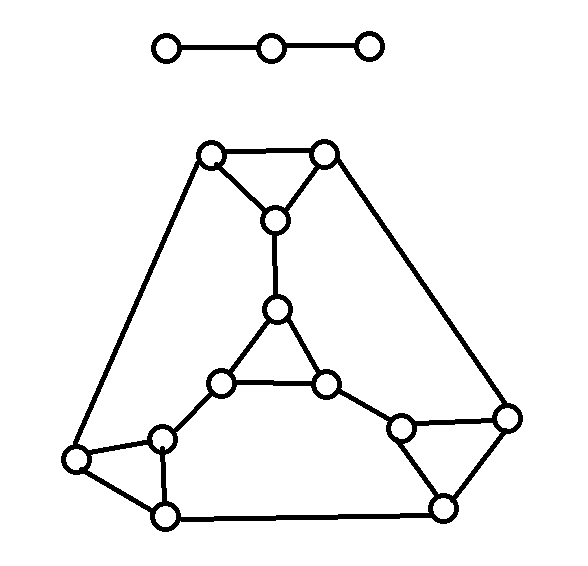
\includegraphics[width=0.3\textwidth]{./pics/graph2.png}

Το πρώτο είναι ακμομεταβατικό, αλλά όχι κορυφομεταβατικό, αφού δεν είναι κανονικό.
\newline
Το δεύτερο είναι ουσιαστικά το τετράεδρο με κομμένες τις γωνίες, άρα εύκολα φαίνεται ότι είναι κορυφομεταβατικό. Δεν είναι όμως ακμομεταβατικό, αφού κάποιες ακμές ανήκουν σε τρίγωνο, ενώ άλλες όχι.


\end{enumerate}
\section{Διάφορα}

\begin{enumerate}
   \item[9.7] \emph{$(\star)$ Ποιά είναι η συνεκτικότητα του υπερκύβου
   $r$ διαστάσεων;}

   Θα δείξουμε με επαγωγή ότι $\kappa(Q_r) = r$.

   Για $r = 1$ το $Q_1$ περιέχει μόνο μία ακμή και είναι συνεκτικό.

   Αν ο $Q_{r-1}$ είναι $(r-1)$-συνεκτικός τότε θα δείξουμε ότι
   ο $Q_r = Q_{r-1} \times P_1$ είναι $r$-συνεκτικός.

   Ο $Q_r$ ως γνωστόν αποτελείται από δύο αντίγραφα $A_1, A_2$ του $Q_{r-1}$
   μαζί με τις ακμές που συνδέουν αντίστοιχες κορυφές μεταξύ τους.
   Στο εξής, αν έχουμε μια κορυφή $u \in V(A_1)$ θα συμβολίζουμε
   με $u'$ την κορυφή του $A_2$ με την οποία συνδέεται η $u$ στο
   $Q_r$.

   Θα δείξουμε ότι για οποιεσδήποτε δύο κορυφές $u, v \in V(Q_r)$
   υπάρχουν $r$ εσωτερικώς διακεκριμένα μονοπάτια από την $u$ στην
   $v$ διακρίνοντας τις εξής περιπτώσεις:

   \begin{itemize}
      \item $u, v \in V(A_1)$ (αντίστοιχα και για το $A_2$).

      Από την Ε.Υ. υπάρχουν $r-1$ εσωτερικώς διακεκριμένα μονοπάτια
      από την $u$ στην $v$ που χρησιμοποιούν μόνο ακμές μόνο από το
      $A_1$. Επίσης υπάρχει τουλάχιστον ένα μονοπάτι $P$ μεταξύ των
      $u'$ και $v'$ στο $A_2$ επομένως μπορούμε να δημιουργήσουμε
      το $P' = [u, u'] \cup P \cup [v', v]$ που δεν έχει κοινές κορυφές με
      τα υπόλοιπα $r-1$ εκτός από τα άκρα.

      \item $u \in V(A_1)$ και $v \in V(A_2)$ (ή αντίστροφα).

      Έστω $P_i$ για $i = 1, \ldots, r-1$ τα $r-1$ εσωτερικώς
      διακεκριμένα μονοπάτια μεταξύ των $u$ και $v$ στο $A_1$ και
      $P_i'$ τα αντίστοιχα μονοπάτια στο $A_2$. Συβολίζουμε με
      $x_i$ τον προτελευταίο κόμβο του μονοπατιού $P_i$.

      Με βάση τα μονοπάτια αυτά δημιουργούμε τα παρακάτω $r$
      εσωτερικώς διακεκριμένα μονοπάτια $R_i$:

      \begin{equation*}
         R_i = \left\{
            \begin{array}{cl}
               [u, u']\cup P_1' &, \ i = 1\\
               (P_i \backslash v) \cup [x_i, x_i', v'] &, \ i = 2, \ldots, r-1\\
               P_1 \cup [v, v'] &,\ i = r\\
            \end{array}
            \right.
      \end{equation*}

   \end{itemize}

	\item[9.8] \emph{$(\star)$ Αν για κάποιο γράφημα $G$ ισχύει ότι $m(G)>n(G)+3$ τότε το $G$ περιέχει δύο ακμοδιακεκριμένους κύκλους.}

Έστω ότι το ζητούμενο δεν ισχύει και θεωρούμε το αντιπαράδειγμα με το ελάχιστο $n(G)$ και δευτερευόντως με το ελάχιστο $m(G)$. Αυτό σημαίνει ότι $m(G)=n(G)+4$, αφού διαφορετικά μπορούμε να διαγράψουμε
ακμές διατηρώντας τη σχέση $m(G)\geq n(G)+4$.
\newline
Προφανώς δεν μπορεί να υπάρχει κύκλος μεγέθους το πολύ $4$, γιατί τότε διαγράφοντας τις ακμές του θα μείνουν τουλάχιστον $n(G)$ ακμές, 
άρα θα έχουμε κύκλο που δεν περιέχει καμία από αυτές τις το πολύ $4$ ακμές. Δηλαδή θα 
έχουμε $2$ ακμοδιακεκριμένους κύκλους, άτοπο.
\newline
Τώρα, αν υπάρχουν κόμβοι με βαθμό το πολύ $1$, διαγράφοντάς τους διατηρείται η ανισότητα $m(G)>n(G)+3$, το οποίο είναι
άτοπο. Επιπλέον, αν υπάρχει κόμβος με βαθμό $2$, τότε διαλύοντάς τον διατηρείται η ανισότητα $m(G)>n(G)+3$ και δεν έχει προστεθεί κανένας επιπλέον κύκλος. Επίσης η ακμή 
που προέκυψε δεν μπορεί να είναι παράλληλη
γιατί τότε πριν τη διάλυση θα υπήρχε τρίγωνο. 
Από τα παραπάνω μπορούμε να υποθέσουμε ότι $\delta (G)\geq 3$. Επιπλέον, έχουμε ότι $n(G)+4 = m(G)\geq \frac{3}{2} n(G)$, άρα $n(G)\leq 8$. 
\newline
Έστω ο ελάχιστος κύκλος $C$, ο οποίος εξ' ορισμού 
δεν θα έχει χορδές.
Παίρνοντας 3 γειτονικές στον κύκλο κορυφές, παρατηρούμε κανένα ζευγάρι αυτών
δεν μπορεί να έχει κοινό γείτονα έξω από τον κύκλο, γιατί τότε θα σχηματιζόταν κύκλος με το πολύ $4$ κορυφές. Άρα υπάρχουν τουλάχιστον $3$
κορυφές έξω από τον κύκλο και άρα ακριβώς $5$ κορυφές μέσα στον κύκλο. Επειδή κάθε δύο κορυφές στον κύκλο απέχουν το πολύ 2 πάνω στον κύκλο, δεν μπορεί να υπάρχουν 2 κορυφές του με κοινό γείτονα έξω
από τον κύκλο γιατί θα σχηματιζόταν κύκλος με το πολύ $4$ κορυφές. Άρα υπάρχουν τουλάχιστον $5$ κορυφές έξω από τον κύκλο, δηλαδή τουλάχιστον $10$ κορυφές συνολικά. Αυτό είναι άτοπο γιατί έχουμε δείξει
ότι υπάρχουν το πολύ $8$ κορυφές.
Συνεπώς το ζητούμενο ισχύει.


   \item[9.9] \emph{$(\star)$ Κάθε $3$-συνεκτικό μη διμερές γράφημα έχει τουλάχιστον $4$ περιττούς κύκλους.}
\begin{proof}
	Εφόσον το γράφημα δεν είναι διμερές, θα έχει περιττό κύκλο. Έστω ο ελάχιστος περιττός κύκλος. Προφανώς αυτός δεν θα έχει χορδές, αφού έτσι θα υπήρχε ακόμα μικρότερος περιττός κύκλος (εφόσον
	κάθε χορδή χωρίζει τον κύκλο σε έναν άρτιο και έναν περιττό). Επιπλέον, θα υπάρχει κορυφή $u$ εξωτερική του κύκλου $C$, 
	αφού γνωρίζουμε ότι ο κύκλος δεν είναι $3$-συνεκτικό γράφημα. Από το Λήμμα \ref{lm9.9.1}, υπάρχουν 3 εσωτερικώς διακεκριμένα μονοπάτια από την $u$ σε διαφορετικές κορυφές του $C$. Έστω 
	$u\equiv P_1^i,P_2^i...,P_{k_i}^i$ για $i\in [1,3]$ αυτά τα τρία μονοπάτια. Για κάθε ζεύγος αυτών, σχηματίζονται δύο κύκλοι. Χωρίς βλάβη της γενικότητας για τα $1$ και $2$, ακολουθούμε το
	μονοπάτι $P^1$, κινούμαστε πάνω στον κύκλο προς την κορυφή $P_{k_2}^2$ (έχουμε δύο τρόπους να το κάνουμε αυτό) και στη συνέχεια ακολουθούμε το μονοπάτι $P^2$ ανάποδα. Καθώς οι δύο εναλλακτικές
	διαδρομές πάνω στον κύκλο τον καλύπτουν ολόκληρο, τα μήκη τους θα έχουν διαφορετικό 
	υπόλοιπο $\mod 2$, άρα τουλάχιστον ένας από τους δύο κύκλους που ορίσαμε θα είναι περιττός.
	Αυτό σημαίνει ότι για κάθε ζευγάρι μονοπατιών $P^i$,$P^j$ έχουμε βρει έναν περιττό κύκλο. Αν σε αυτούς
	μετρήσουμε και τον $C$, έχουμε συνολικά βρει $4$ περιττούς κύκλους.
\end{proof}

\begin{lm}
   \label{lm9.9.1}
	Έστω $k$-συνεκτικό γράφημα, κύκλος $C$ και κορυφή $u$ που δεν ανήκει στον κύκλο. Τότε υπάρχουν $\min(|C|,k)$ εσωτερικώς διακεκριμένα μονοπάτια από την $u$ προς διαφορετικές κορυφές του
	κύκλου $C$.
\end{lm}
\begin{proof}
	Έχει αποδειχθεί στην πρώτη σειρά ασκήσεων.
\end{proof}
	
\end{enumerate}

\end{document}
